\chapter{Domain Analysis}
Given the complexity of the domain, it was decided to use Event Storming to become familiar with the terminologies and workflows typical of the domain. The adoption of this activity was also justified by having real domain experts available to explain to us the current business processes. In addition, using this approach it was possible to bring together managers from different areas, who collaborated to correctly define the dynamics and problems concerning their communication.

\section{Subdomains}
These are the subdomains that emerged from the Event Storming process:
\begin{itemize}
    \item Production Planning: creates the daily production planning
    \item Milk Planning: estimates the amount of milk to order each week
    \item Stocking: manages the packaging of cheeses and their stocking
    \item Restocking: orders the milk and keeps track of the available quantity of milk
    \item Client Orders: handles and fulfills the orders made by clients
    \item Production: tracks the cheeses' production process
    \item Pricing: calculates the price for every order considering the specific client
\end{itemize}

We proceeded with this exploration of the domain by individuating the subdomains where digital twins would have been crucial to help the processes.
The two subdomains we selected were \textit{Milk Planning} and \textit{Stocking} \ref{img:event-storming}.
The decision was made considering the added value that the digital twins could bring to the processes (this aspect will be explored in the\ref{sec:dt-motivations} section) and the fact that the two subdomains were quite complex.
The \textit{Stocking} subdomain is the one that manages the quality assurance of the cheeses, which is a crucial process for the company.
The \textit{Milk Planning} subdomain is the one that estimates the amount of milk to order each week, which is a process that is very important for the company's financial health.

\begin{figure}[H]
    \centering
    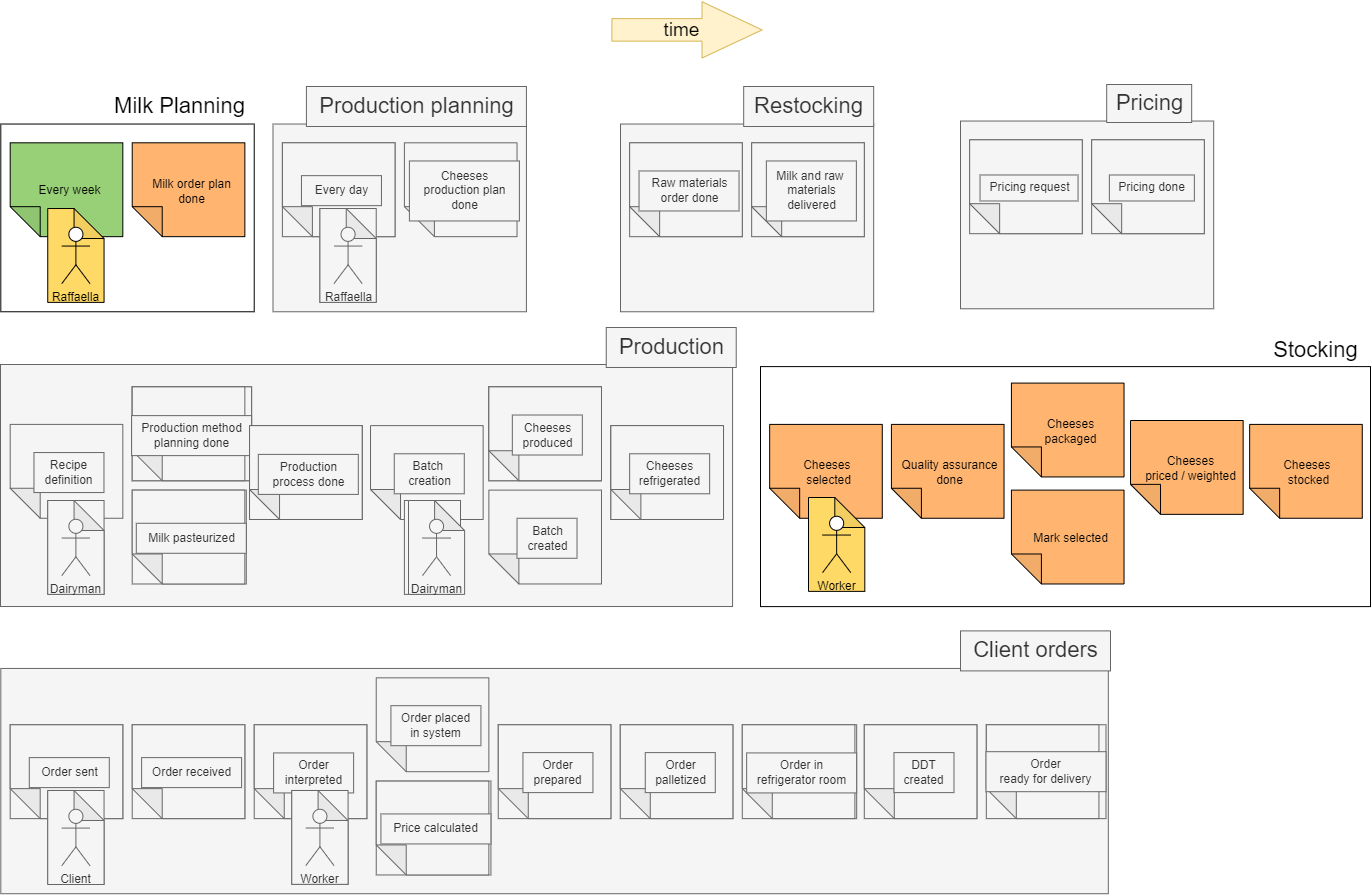
\includegraphics[width=\textwidth]{img/event-storming.png}
    \caption{Event storming result. The image highlights the two subdomains we selected for interacting with the digital twins}
    \label{img:event-storming}
\end{figure}

\section{Digital Twins - motivations}\label{sec:dt-motivations}
This section will describe the digital twins that were chosen to be implemented in the project and the motivations behind the choice of inserting them in this context.

\subsection{Milk Tank Digital Twin}
The digital twin we individuated for the Milk Planning subdomain is the Milk Tank Digital Twin.
The main motivation for the adoption of this digital twin is the need to have real-time monitoring of the milk quantity and quality in the tanks.

The digital twin will be able to provide the Milk Planning subdomain with information about the milk quantity in the tanks, which will be used to estimate the amount of milk to order each week.

Moreover, the tank will provide information about the pH and the temperature of the milk, which will be used to decide if the milk is suitable for the production of a specific cheese.

\subsection{Packaging Machine Digital Twin}
The packaging machine is a very important machine in the production process as well as very complex and expensive.
It is also fairly prone to breakdowns and this can cause a lot of problems in the production process.

For these reasons, the introduction of a digital twin that can monitor the machine and predict when it will break down can be considered crucial.

\subsection{Scale Digital Twin}
We decided to implement a digital twin for the Scale since there are many scenarios in which it could be useful.
The scale could be used to monitor the weight of the packages and detect if there are any anomalies. If so, it may be a sign of a problem in the packaging process (e.g. deformed molds).

\subsection{Metal detector Digital Twin}
The metal detector is a device that is used to detect metal objects in packages. It is used to ensure that the packages are free of metal objects, which could be dangerous for the consumer.
The digital twin of the metal detector will be able to detect if there are any anomalies in the packages.

The detection of metallic components is, however, very rare and could imply that the machine to make cheese might have deteriorated. So, along with checking the batch where the anomaly is detected, a check of the machine could also be performed.


\section{Supporting bounded contexts}
Having introduced digital twins we noticed that other subdomains or bounded contexts were needed in order to support their functioning.
In particular, we identified the following bounded contexts:
\begin{itemize}
    \item Alerts: manages the alerts sent by the digital twins
    \item Maintenance: manages the maintenance of the Packaging Machine digital twin
    \item Reporting: manages the reports sent by the Scale and the Metal Detector digital twins
\end{itemize}

The \textit{Alerts} bounded context is responsible for collecting the fault messages coming from the digital twins, storing them and notifying the responsible people.

For instance, \textit{Milk Tank} would notify any anomaly in the milk quality (pH or temperature values out of range);
\textit{Packaging Machine} would notify any anomaly in the machine status (e.g. a broken part) and \textit{Scale} and \textit{Metal Detector} would notify any anomaly in the weight or the presence of metal.

The \textit{Maintenance} bounded context was mainly introduced to predict the maintenance of the Packaging Machine digital twin but its use could be extended to other machines.

Finally, the \textit{Reporting} bounded context was introduced to collect the reports sent by the Scale and the Metal Detector digital twins and to do some basic analysis on this data.
Given its simplicity and the fact that it doesn't add business differentiation, this bounded context will be outsourced to a third-party company.

The figure\ref{img:subdomains-dt} shows the bounded contexts and the digital twins that interact with them.

\begin{figure}[H]
    \centering
    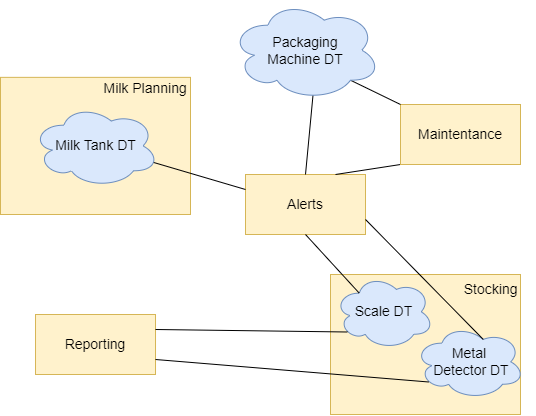
\includegraphics[width=\textwidth]{img/subdomains-dt.png}
    \caption{The supporting bounded contexts and their interactions with the digital twins}
    \label{img:subdomains-dt}
\end{figure}

\section{Business differentiation}
We then proceeded to have a more in-depth analysis of each subdomain to determine their business differentiation and to do a first estimate of the model's complexity. The following considerations were made:
\begin{itemize}
    \item Production Planning and Milk Planning are to be considered core subdomains since they can be decisive in order to optimize the efficiency of the factory
    \item the Milk Planning subdomain can be seen as a big-bet subdomain since it has the potential to significantly disrupt the market if implemented in such a way that can predict trends and spikes in orders
    \item the Reporting subdomain is considered as outsourced since it is not a core subdomain and it is not a big-bet subdomain either. It is also not a subdomain that can be considered a differentiator for the company.
    \item the remaining subdomains introduce a lower amount of business differentiation, so they are to be considered as supporting subdomains
\end{itemize}

We gathered these pieces of information and compiled the following core domain chart:

\begin{figure}[H]
    \centering
    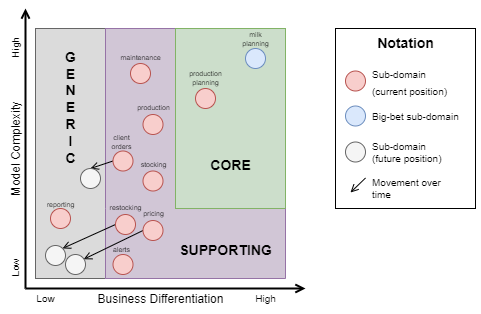
\includegraphics[width=\textwidth]{img/core-domain-chart.png}
    \caption{The core domain chart of the identified subdomains}
    \label{img:core-domain-chart}
\end{figure}
